\pdfoutput=1
\documentclass[11pt]{article}
\textwidth=5.00in
\textheight=7.4in
\topmargin=30pt
\evensidemargin=0pt
\oddsidemargin=55pt
\headsep=17pt
\parskip=.5pt
\parindent=12pt
\font\smallit=cmti10
\font\smalltt=cmtt10
\font\smallrm=cmr9

\usepackage{amssymb,latexsym,amsmath,amsthm}
\usepackage{graphicx}
\usepackage[hidelinks]{hyperref}

\makeatletter
\renewcommand\section{\@startsection {section}{1}{\z@}
{-30pt \@plus -1ex \@minus -.2ex}
{2.3ex \@plus.2ex}
{\normalfont\normalsize\bfseries\boldmath}}
\renewcommand\subsection{\@startsection{subsection}{2}{\z@}
{-3.25ex\@plus -1ex \@minus -.2ex}
{1.5ex \@plus .2ex}
{\normalfont\normalsize\bfseries\boldmath}}
\renewcommand{\@seccntformat}[1]{\csname the#1\endcsname. }
\makeatother

\theoremstyle{plain}
\newtheorem{theorem}{Theorem}
\newtheorem{lemma}{Lemma}
\newtheorem{proposition}{Proposition}
\newtheorem{corollary}{Corollary}
\theoremstyle{definition}
\newtheorem{definition}{Definition}
\newtheorem{example}{Example}
\newtheorem{conjecture}{Conjecture}
\theoremstyle{remark}
\newtheorem{remark}{Remark}

\newcommand{\seqnum}[1]{\href{https://oeis.org/#1}{\rm \underline{#1}}}

\begin{document}

% 2020 Mathematics Subject Classification: Primary 11B83; Secondary 11A25, 60J10.
% Keywords: Collatz conjecture, 2-adic valuation, stopping time, dynamical iteration.
 
\begin{center}
\uppercase{\bf\boldmath Residue Classes and Stopping Times for an Accelerated Collatz Map} 
\vskip20pt
{\bf Michael Goldapp}\\
{\smallit Ostfalia University of Applied Sciences, Wolfenbuettel, Germany}\\
{\tt mi.goldapp@ostfalia.de}
\end{center}

\vskip30pt

\centerline{\bf Abstract}
\noindent
We introduce a modification of the Collatz function that shortens trajectories, reduces peak values, and suggests 
that the average stopping time remains bounded as the starting value grows. 
For a majority of starting values, a single step suffices to reach a strictly smaller integer. 
We provide probabilistic estimates based on a first-passage heuristic model, 
a linear composition formula, and detailed analyses for $n = 2^m - 1$ and $n = 10^m + j$.
The principal rigorous result of this paper is an eventual stabilization theorem for the stopping times 
of integers of the form $10^m + j$. 
The remaining sections develop the arithmetic structure of the accelerated map and present numerical 
and heuristic evidence concerning starting values.

\pagestyle{myheadings}
 
\thispagestyle{empty}
\baselineskip=12.875pt
\vskip30pt

\section{Introduction}

The $3x+1$ problem or Collatz problem concerns the iteration of the Collatz function $C: \mathbb{N} \to \mathbb{N}$, defined as
\begin{displaymath}
C(x) = \begin{cases}
3x+1, & \text{if $x \equiv 1$ (mod $2$);}\\
x/2, & \text{if $x \equiv 0$ (mod $2$).}
\end{cases}.
\end{displaymath}

The classical conjecture is as follows.
\begin{conjecture}[Collatz Conjecture]
Starting from any positive integer $n$, iterations of the function $C(n)$ will eventually reach the number $1$ and thereafter cycle through the values $1, 4, 2, 1, \dots$.
\end{conjecture}

Terras \cite{Ter76} and Everett \cite{Ev77} introduced the compressed function
\begin{displaymath}
T(x) = \begin{cases}
(3x+1)/2, & \text{if $x \equiv 1$ (mod $2$);}\\
x/2, & \text{if $x \equiv 0$ (mod $2$),}
\end{cases}.
\end{displaymath}
which combines two $C(n)$ steps whenever $n$ is odd. The standard total stopping time for $n$ under $C(n)$ is recorded in sequence \seqnum{A006577}. Another variation is the Syracuse function $S(x)$, defined for odd $x$ by
\begin{displaymath}
S(x) = (3x+1)/2^{\nu_2(3x+1)} ,
\end{displaymath}
where $\nu_2(n)$ denotes the $2$-adic valuation of $n$ (the highest power of $2$ dividing $n$). \par
Lagarias \cite{Lag-B1, Lag-B2, Lag10} provided comprehensive overviews of this research area. \par
The {\em $3x+1$} conjecture has so far been verified computationally for all 
$n < 2^{71} \approx 2.3611 \cdot 10^{21}$
(Barina \cite{Bar25}).\par
 
This paper introduces a further modification of the Collatz function that produces shorter trajectories. 
We refer to it as the { \em accelerated Collatz function}.
The approach taken here is based on the $2$-adic structure of $n+1$ for odd $n$.
Any odd integer $n$ can be uniquely written as 
\begin{displaymath}
n = r \cdot 2^k - 1, \quad \text{with $r$ odd and $k = \nu_2(n+1) \ge 1$.}
\end{displaymath}
Applying $T(x)$ repeatedly $k$ times to $n$ yields
\begin{displaymath}
T^k(n) = 3^k r - 1.
\end{displaymath}
Since $r$ is odd and $k \ge 1$, the intermediate result $T^k(n)$ is an even number that can be divided by $2$ one or more times. 
Setting $q = \nu_2(3^k r - 1)$, all of these divisions by $2$ can be incorporated into a single step.

\section{Definition and Basic Properties}

We now give the central definition.
\begin{definition}
The accelerated Collatz function $\bar{c}: \mathbb{N} \to \mathbb{N}$ is defined by
\begin{displaymath}
\bar{c}(n) = \begin{cases}(3^k r - 1)/2^q, & \text{for odd $n = r \cdot 2^k - 1$, with $k = \nu_2(n+1)$}\\
& \text{and $q = \nu_2(3^k r - 1)$;}\\
 n/2^k, & \text{for even $n = r \cdot 2^k$, with $k = \nu_2(n)$.}
\end{cases}.
\end{displaymath}
\end{definition}

We let $\mathcal{L}(\mathcal{F}, n_0)$ denote the number of iterations required for the trajectory under a function $\mathcal{F}$. 
The initial value $n_0$ is not counted.
It is sufficient to investigate the behavior until a smaller value $n_t < n_0$ is reached. Then $n_t$ can be regarded as the new starting point until $1$ is reached.

\subsection{Basic Properties}
\begin{enumerate}
\item \emph{Always odd.} For any $n \in \mathbb{N}$, the value $\bar{c}(n)$ is always an odd integer because the denominator removes all factors of $2$.
\item \emph{Fixed point at 1.} Whereas $C(n)$ has the cycle $1\rightarrow 4\rightarrow 2 \rightarrow 1$ and $T(n)$ has the $1 \to 2 \to 1$ loop, the accelerated function satisfies 
$\bar{c}(1) = 1$ as a fixed point.
\item \emph{Three out of four numbers stop in one step.} The definition preserves the property that each even number immediately leads to a smaller number. Furthermore, for $n \equiv 1$ (mod $4$), we have $k = 1$ and $n = 2r - 1$, so $\bar {c}(r \cdot 2^1 - 1) = (3 r  - 1)/2^q \le (3 r  - 1)/2 < 3/2~r  < n$. 
Thus, three out of four numbers stop after a single step, leaving only $n \equiv 3$ (mod $4$) for further investigation, excluding the trivial $n=1$.
\item \emph{Different first stopping values.}

For $n_0 = 10087$, the trajectories for $C(n)$ and $T(n)$ both reach $13667$ and eventually 
map to $7688$, whereas $\bar{c}(n)$ maps $13667$ directly to $961$. Both $7688$ and $961$ are smaller
 than $n_0$, but not identical. This occurs because $\bar{c}(n)$ always applies the full divisor $2^q$.
 
\item \emph{Reduced maximum excursion.} For $n_0 = 27$, the maximal value in the $T(n)$ sequence is $3644$, which reduces to $911$ under $\bar{c}(n)$. Kontorovich and Lagarias \cite{KL09} defined the maximum excursion ratio $\rho$ as
\begin{displaymath}
\rho(n_0) = \max_{j \ge 1} \frac{\log T^j(n_0)}{\log n_0},
\end{displaymath}
which exceeds $2$ when $n_0^2$ is exceeded. 
Of the eight numbers previously listed in \seqnum{A365482} exceeding $\rho > 2$ under $T(n)$ (with corresponding peak values listed in \seqnum{A365483}),  
only three of them still have an excursion ratio greater than $2$ under $\bar{c}(n)$, 
namely $n_0 = 27$, $3716509988199$, and $1980976057694848447$, 
the last of which was originally found by Oliveira e Silva \cite{OeS09}. \par
There are three even larger numbers with that property, under both $T(n)$ and $\bar{c}(n)$:
$2641301410259797929$, $2971464086542272671$ and \par $3961952115389696895$ (all with 19 digits). \par
The starting values giving rise to trajectory peaks without necessarily exceeding $\rho > 2$ are the path records \seqnum{A006884}. 
\end{enumerate}

\section{Acceleration}

\subsection{Examples}

Starting with $n_0 = 27$, the trajectory for $C(n)$ takes $111$ steps to reach $1$ (\seqnum{A006577}), and $96$ steps to reach the smaller $n_t = 23$. With $T(n)$ it takes $59$ steps to reach $n_t = 23$, while with $\bar{c}(n)$ only $15$ steps suffice. 
This corresponds to an acceleration factor of approximately $3.9$ relative to $T$, or $6.4$ relative to $C$.

Below is the complete trajectory for $T(n)$, with the values calculated by $\bar{c}(n)$ highlighted in boldface:

\medskip
\noindent
\textbf{27}, 41, 62, \textbf{31}, 47, 71, 107, 161, 242, \textbf{121}, 182, \textbf{91}, 137, 206, \textbf{103}, 155, 233, 350, \textbf{175}, 263, 395, 593, 890, \textbf{445}, 668, 334, \textbf{167}, 251, 377, 566, \textbf{283}, 425, 638, \textbf{319}, 479, 719, 1079, 1619, 2429, 3644, 1822, \textbf{911}, 1367, 2051, 3077, 4616, 2308, 1154, \textbf{577}, 866, \textbf{433}, 650, \textbf{325}, 488, 244, 122, \textbf{61}, 92, 46, \textbf{23}.
\medskip

Starting with $n_0 = 1023$, $C(n)$ takes $62$ steps to reach $1$ ($29$ to reach a smaller number), and $T(n)$ takes $18$ steps. The function $\bar{c}(n)$ achieves this in only $2$ steps: $1023, 7381, 173$.

\subsection{Acceleration Factor}

A single application of $\bar{c}(n)$ corresponds to $k$ steps of $S(n)$, $k+q$ steps of $T(n)$, and $2k+q$ steps of $C(n)$.

The relevant expected values are summarized in the following proposition.
\begin{proposition}\label{prop:acceleration}
The expected values of $k$ and $q$ for $n \equiv 3$ (mod $4$) are given by
\begin{displaymath}
\mathbb{E}(k \mid n \equiv 3 \pmod  8) = 2, \quad \mathbb{E}(k \mid n \equiv 7 \pmod  8) = 4, \quad \mathbb{E}(q) = 2.
\end{displaymath}
Consequently, the average acceleration factor $F = 2k+q$ relative to $C(n)$ is $6$ for $n \equiv 3 \bmod  8$  and $10$ for $n \equiv 7 \bmod  8$.
\end{proposition}

\begin{proof}
For $n \equiv 3$ (mod $8$), $n+1 = 4(2a+1)$, so $k = \nu_2(n+1) = 2$. \par
For $n \equiv 7$ (mod $8$), $n+1 = 8(a+1)$, so $k = 3 + \nu_2(a+1)$. 
Since $\mathbb{P}(\nu_2(m) = j) = 2^{-(j+1)}$ for $j\ge 0$, in terms of asymptotic natural density, $\mathbb{E}(\nu_2(m)) = 1$. 
Thus, $\mathbb{E}(k \mid n \equiv 7 \text{ (mod } 8\text{)}) = 3 + 1 = 4$.

For fixed $k$ and $j \ge 1$, $3^k r \equiv 1 + 2^j$ (mod $2^{j+1}$) has a unique odd solution $r$ (mod $2^{j+1}$). 
Hence, $q$ follows the geometric distribution $\mathbb{P}(q = j) = 2^{-j}$ for $j \ge 1$, and its expected value is $\mathbb{E}(q) = \sum_{j=1}^{\infty} j / 2^j = 2$.
\end{proof}

\section{Single Steps and Linear Composition}

For fixed $n$, $\bar{c}(n)$ acts linearly as $\bar{c}(n) = A(k,q) \cdot n + c(k,q)$, where
\begin{displaymath}
A(k,q) = \frac{3^k}{2^{k+q}}, \qquad c(k,q) = \frac{3^k - 2^k}{2^{k+q}}.
\end{displaymath}
The multiplier $A(k,q) > 1$ when $q \le \lfloor \alpha k \rfloor$ with $\alpha = \log_2 3 - 1 \approx 0.58496$.

Accumulating $t$ steps yields $n_t = (3^{K_t} n_0 + B_t)/2^{S_t}$, where 
\begin{displaymath}
K_t = \sum_{i=0}^{t-1} k_i ~~,~~  Q_t = \sum_{i=0}^{t-1} q_i~~ ,~~  S_t = K_t + Q_t,
\end{displaymath}
and $B_t$ is recursively defined by $B_0 = 0$ and $B_{i+1} = 3^{k_i} B_i + (3^{k_i} - 2^{k_i}) 2^{S_i}$.
The recursive sequence $B_t$ can be evaluated efficiently in $O(t)$ arithmetic operations via a Horner-like evaluation scheme during the step-by-step composition.
From $n_t$ as an odd integer, it follows that $3^{K_t} n_0 + B_t \equiv 2^{S_t} \pmod{2^{S_t+1}}$. 
Inverting $3^{K_t}$ specifies a unique start value residue class $n_0 \equiv 3^{-K_t} (2^{S_t} - B_t) \pmod{2^{S_t+1}}$.
For example, $n_0 = 27$ reaching $n_t = 23$ gives $K_t = 37, Q_t = 22, S_t = 59$, and $B_t = 1100931843921811423$. 
Substitution into the composition formula gives $n_t=23 < 27=n_0$.
Moreover, $Q_t = 22 > 37 \alpha \approx  21.643$, so the cumulative multiplicative factor is less than $1$.

\section{Large Start Values and Trajectory Dynamics}

\subsection{One Step Suffices in Many Cases}

For $n \equiv 3$ (mod $4$), a step decreases $n$ when $q \ge \lfloor \alpha k \rfloor + 1$. The probability of an immediate reduction is
\begin{displaymath}
\mathbb{P}(n_1 < n_0) = \sum_{k=2}^{\infty} 2^{1-k} \cdot 2^{-\lfloor \alpha k \rfloor} \approx 0.42745.
\end{displaymath}
This explicit single-step stopping probability corresponds to the exact summation with $\alpha = \log_2 3 - 1$, 
demonstrating that the immediate descent rate is strictly governed by the underlying $2$-adic distribution. \par
Thus, roughly $42.7$ percent of all starting values $n \equiv 3$ (mod $4$) result in a smaller number in the first step. 
This agrees with computational experiments, which give  $42.745$ percent for all $n_0 < 10^7$ for $n_0 \equiv 3$ (mod $4$).

\subsection{Average Number of Steps for Large \texorpdfstring{$n$}{n}}

Numerical experiments indicate that the arithmetic mean of $\mathcal{L}(\bar{c}, n)$ taken for all $n<10^m$, $n \equiv 3$ (mod $4$), approaches 
a constant close to $2.5$ as $m$ increases. 
Figure \ref{fig1} displays the corresponding numerical means.

\begin{figure}[ht]
\begin{center}
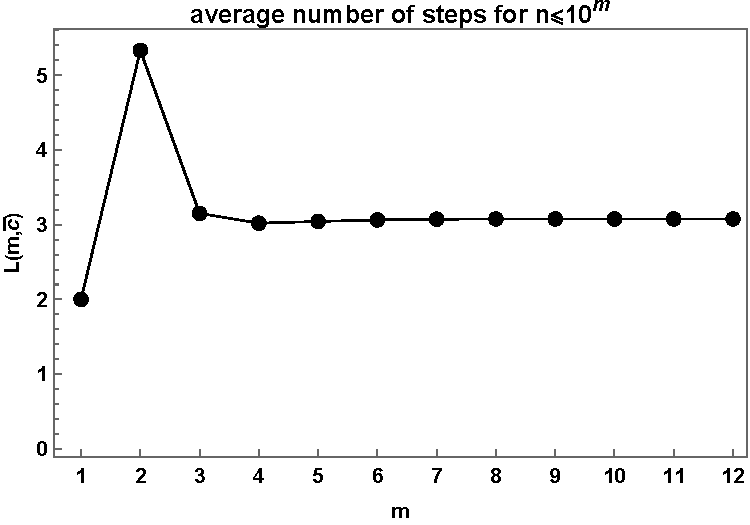
\includegraphics[width=4in]{figure1.pdf}
\end{center}
\caption{Average number of steps to reach a smaller number for $n < 10^m$, $n \equiv 3$ (mod $4$).}
\label{fig1}
\end{figure}

We use the following renewal approximation. After each non-stopping
iteration, the residue data determining the next pair $(k,q)$ are
treated as newly sampled from the same asymptotic distribution and
as independent of the preceding steps. If $p$ denotes the probability
that one iteration produces a value below the current reference value,
then the corresponding first-passage time is modeled by a geometric
random variable:
\begin{displaymath}
\mathbb{P}(t=s)=(1-p)^{s-1}p,\qquad \mathbb{E}(t)=\frac{1}{p}.
\end{displaymath}
This is a heuristic stochastic model; independence of successive Collatz iterates is not asserted.

For starting values $n\equiv3\pmod8$, the model gives $p=1/2$ and
therefore
\begin{displaymath}
\mathbb{E}(t)\approx 2.
\end{displaymath}
For starting values $n\equiv7\pmod8$, the estimated continuation
probability is
\begin{displaymath}
r=1-4\sum_{k=3}^{\infty} 2^{-\lfloor k(\alpha+1)\rfloor} \approx0.6451.
\end{displaymath}
Thus, the corresponding stopping probability is
$p=1-r\approx0.3549$, giving
\begin{displaymath}
\mathbb{E}(t)\approx\frac{1}{0.3549}\approx2.82.
\end{displaymath}
The slight discrepancy between this heuristic estimate and the observed empirical mean ($3.07692$) for $n \equiv 7 \pmod 8$ 
arises from a weak correlation between consecutive iterates, which partially violate the idealized independence assumption.

Replacing $r$ by the rough approximation $2/3$ gives the simpler estimate $\mathbb{E}(t)\approx 3$.
The renewal approximation is intentionally simplified and does not reproduce the numerical means exactly. 
For $n<10^{12}$ with $n\equiv 3$ (mod $4$), the observed arithmetic mean is $2.49266$.
The corresponding means in the residue classes $3$ and $7$ modulo $8$ are $1.90838$ and $3.07692$, respectively.

\subsection{Irregular Growth for \texorpdfstring{$n = 2^m - 1$}{n=2\^m-1}}

For $n = 2^m - 1$, $k_1 = m$. By the lifting-the-exponent lemma \cite{Cu-Sa, Pava}, $q_1 = 1$ for odd $m$, and $q_1 = 2 + \nu_2(m)$ for even $m$.

The residue classes $n \equiv -1 $ (mod ${2^m}$) force large initial growth $A(k,q)$, 
making these residue classes natural candidates for unusually long trajectories.
This  does not assert that these residue classes
produce the globally longest trajectories.\par
Figure \ref{fig2} compares these stopping times with the linear heuristic.

\begin{figure}[ht]
\begin{center}
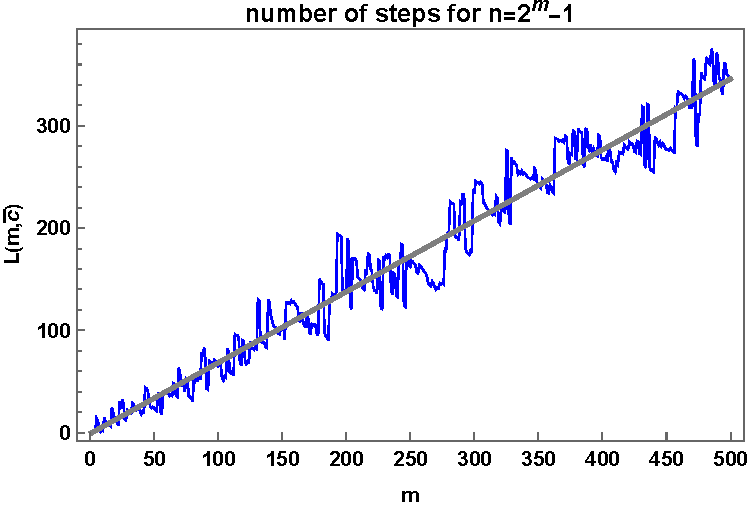
\includegraphics[width=4in]{figure2.pdf}
\end{center}
\caption{Number of steps for $n = 2^m - 1$, overlaid with $0.7047\, m$.}
\label{fig2}
\end{figure}


To estimate the number of iterations following the initial growth
step, we use a simplified effective-drift model. We take $k_i=2$,
as in the residue class $n_i\equiv 3$ (mod $8$), and use the geometric
valuation model $\mathbb{E}(q_i)=2$. Since
\begin{displaymath}
\log h_i=k_i\log(3/2)-q_i\log2,
\end{displaymath}
this gives
\begin{displaymath}
\mathbb{E}[\log h_i] \approx 2\log(3/2)-2\log2=\log(9/16).
\end{displaymath}
This value is an effective heuristic drift, not an unconditional
expectation over all odd Collatz iterates.

The logarithmic height gained in the first step is approximately
\begin{displaymath}
m\log(3/2)-q_1\log2.
\end{displaymath}
Dividing this gain by the magnitude of the assumed negative drift
$\log(16/9)$ gives
\begin{displaymath}
\mathcal{L}(\bar c,2^m-1)\approx1+\frac{m\log(3/2)-q_1\log2}{\log(16/9)}.
\end{displaymath}
Hence,
\begin{displaymath}
\mathcal{L}(\bar c,2^m-1)\approx0.7047\,m-1.2047\,q_1+1.
\end{displaymath}
 

\subsection{Bounded Growth for \texorpdfstring{$n = 10^m + j$}{n=10\^m+j}}

We now give a sufficient condition under which
$\mathcal{L}(\bar c,10^m+j)$ is eventually constant. The result applies
whenever the cumulative multiplier associated with the trajectory of
$j$ becomes smaller than $1$.


\begin{lemma}\label{lem:prefix-stability}
Let $j$ be a fixed odd integer, $n_0 = j$, $N_0 = 10^m + j$, and $S_t = \sum_{i=1}^t (k_i + q_i)$. If $m \ge S_t + 1$, then $N_0$ and $n_0$ share identical parameter pairs $(k_i, q_i)$ for $1 \le i \le t$, and
\begin{displaymath}
\bar{c}^t(10^m + j) = \frac{3^{K_t}}{2^{S_t}} 10^m + \bar{c}^t(j).
\end{displaymath}
\end{lemma}

\begin{proof}
By induction on $t$. For $t=0$, $N_0 \equiv n_0$ (mod ${2^m})$. Assuming coincidence for $i$ steps, $N_i - n_i = 3^{K_i} 2^{m - S_i} 5^m$, so $\nu_2(N_i - n_i) = m - S_i$. If $m \ge S_t + 1$, then $m - S_i \ge k_{i+1} + q_{i+1} + 1$, preserving the parameter pair for step $i+1$.
\end{proof}

We obtain the following consequence.
\begin{corollary}\label{cor:stopping-stability}
Let $j$ be a fixed odd positive integer, and let $(k_i,q_i)$ be the parameter pairs generated by the trajectory of $j$. Define
\begin{displaymath}
K_t=\sum_{i=1}^t k_i,\qquad S_t=\sum_{i=1}^t(k_i+q_i), \qquad a_t=\frac{3^{K_t}}{2^{S_t}}.
\end{displaymath}
Assume that the set $\{t\ge1:a_t<1\}$ is nonempty, and define
\begin{displaymath}
\tau=\min\{t\ge1:a_t<1\}.
\end{displaymath}
Then there exists an integer $M(j)$ such that
\begin{displaymath}
\mathcal{L}(\bar c,10^m+j)=\tau
\end{displaymath}
for every $m\ge M(j)$.
\end{corollary}

\begin{proof}
Since a positive power of $3$ cannot equal a positive power of $2$, we have $a_i\neq1$ for every $i\ge1$. 
Hence, by the minimality of $\tau$,
\begin{displaymath}
a_i>1\quad(1\le i<\tau), \qquad a_\tau<1.
\end{displaymath}
Choose $m$ sufficiently large that Lemma \ref{lem:prefix-stability} applies through step $\tau$. Then
\begin{displaymath}
\bar c^i(10^m+j)-(10^m+j) = (a_i-1)10^m+\bigl(\bar c^i(j)-j\bigr).
\end{displaymath}
For each $i<\tau$, the coefficient $a_i-1$ is positive. Hence, for
all sufficiently large $m$,
\begin{displaymath}
\bar c^i(10^m+j)>10^m+j.
\end{displaymath}
At $i=\tau$, the coefficient $a_\tau-1$ is negative, and therefore,
for all sufficiently large $m$,
\begin{displaymath}
\bar c^\tau(10^m+j)<10^m+j.
\end{displaymath}
Thus, the first value below the initial value occurs after exactly
$\tau$ iterations.
\end{proof}

The stabilization threshold can be determined explicitly in the following example.
\begin{example}\label{ex:j31}
For $j=31$, the parameter pairs along the first fourteen iterations
give
\begin{displaymath}
K_{13}=34,\qquad S_{13}=53, \qquad\text{and}\qquad K_{14}=35,\qquad S_{14}=56.
\end{displaymath}
Consequently,
\begin{displaymath}
a_{13}=\frac{3^{34}}{2^{53}}>1,\qquad a_{14}=\frac{3^{35}}{2^{56}}<1.
\end{displaymath}
Thus, $\tau=14$. Since $S_{14}=56$, Lemma \ref{lem:prefix-stability} and Corollary \ref{cor:stopping-stability} imply
\begin{displaymath}
\mathcal{L}(\bar c,10^m+31)=14 \qquad\text{for every }m\ge 57.
\end{displaymath}
A direct calculation gives
\begin{displaymath}
\mathcal{L}(\bar c,10^{55}+31)=15, \qquad \mathcal{L}(\bar c,10^{56}+31)=14.
\end{displaymath}
It follows that the exact stabilization threshold is $m^*=56.$
\end{example}

Figure \ref{fig3} illustrates this stabilization numerically.

\begin{figure}[ht]
\begin{center}
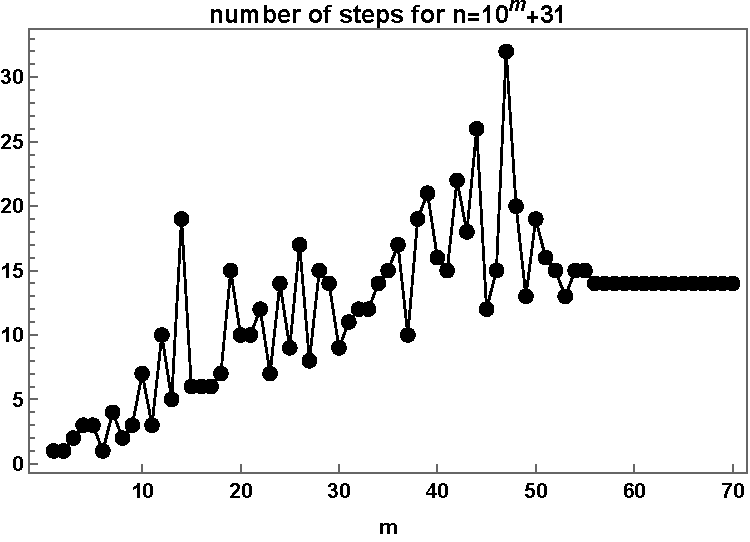
\includegraphics[width=4in]{figure3.pdf}
\end{center}
\caption{Number of steps for $n = 10^m + 31$, showing stabilization at 14 steps for $m \ge 56$.}
\label{fig3}
\end{figure}

\section{Conclusion}

The accelerated Collatz function $\bar{c}(n)$ provides a new tool for studying Collatz dynamics. 
Its use of the  $2$-adic structure of $n+1$ compresses several intermediate steps into a single iteration. 
We derive heuristic estimates for the families $n = 2^m - 1$ and $10^m + j$. 
Numerical experiments and heuristic arguments further suggest that the average stopping time over suitable residue classes may remain bounded.

\section{List of OEIS Sequences}

The sequences referenced in this paper are listed in the On-Line Encyclopedia of Integer Sequences \cite{OEIS}:
\begin{itemize}
\item \seqnum{A006577}: Total stopping time under the Collatz function.
\item \seqnum{A006884}: Trajectory path records in the Collatz problem.
\item \seqnum{A365482}: Path records with maximum excursion ratio greater than 2.
\item \seqnum{A365483}: Corresponding maximum excursion values for \seqnum{A365482}.
\end{itemize}

\begin{thebibliography}{99}\footnotesize

\bibitem{Bar25}
D. Barina, Improved verification limit for the convergence of the Collatz conjecture, {\it J. Supercomput.} {\bf 81} (2025), 810.

\bibitem{Cu-Sa}
S. Cuellar and J. A. Samper, A nice and tricky lemma (lifting the exponent), {\it Math. Reflections} {\bf 3} (2007).

\bibitem{Ev77}
C. J. Everett, Iteration of the number theoretic function $f(2n)=n, f(2n+1)=3n+2$, {\it Adv. Math.} {\bf 25} (1977), 42--45.

\bibitem{KL09}
A. V. Kontorovich and J. C. Lagarias, Stochastic models for the $3x+1$ problem and generalizations, in J. C. Lagarias, ed., {\it The Ultimate Challenge: The $3x+1$ Problem}, Amer. Math. Soc., Providence, RI, 2010, 131--188.

\bibitem{Lag-B1}
J. C. Lagarias, The $3x+1$ problem: an annotated bibliography (1963--1999), in J. C. Lagarias, ed., {\it The Ultimate Challenge: The $3x+1$ Problem}, Amer. Math. Soc., Providence, RI, 2010, 267--341.

\bibitem{Lag-B2}
J. C. Lagarias, The $3x+1$ problem: an annotated bibliography, II (2000--2009), preprint, {\tt arXiv:math/0608208}.

\bibitem{Lag10}
J. C. Lagarias, The $3x+1$ problem: an overview, in J. C. Lagarias, ed., {\it The Ultimate Challenge: The $3x+1$ Problem}, Amer. Math. Soc., Providence, RI, 2010, 3--29.

\bibitem{OeS09}
T. Oliveira e Silva, Empirical verification of the $3x+1$ and related conjectures, in J. C. Lagarias, ed., {\it The Ultimate Challenge: The $3x+1$ Problem}, Amer. Math. Soc., Providence, RI, 2010, 189--207.

\bibitem{OEIS}
OEIS Foundation Inc., The On-Line Encyclopedia of Integer Sequences, \url{https://oeis.org}.

\bibitem{Pava} 
A. Parvardi, Lifting the exponent lemma (LTE), 2011. Available at \url{www.academia.edu/101947929/Lifting_The_Exponent_Lemma_LTE_Version_6}.

\bibitem{Ter76}
R. Terras, A stopping time problem on the positive integers, {\it Acta Arith.} {\bf 30} (1976), 241--252.

\end{thebibliography}

\end{document}

\typeout{get arXiv to do 4 passes: Label(s) may have changed. Rerun}
